\documentclass[11pt]{article}
\usepackage{listings}
\usepackage{graphicx}

\begin{document}
\lstset{language=Matlab}

\title{COMPM012 - Coursework 2}
\author{Esben A. S\o rig}

\maketitle

\section{Fitting with Polynomial Bases}
\begin{itemize}
    \item[a)]
        To fit the data with the polynomial bases $k=1,2,3,4$ we apply each of the polynomial basis to the $x$-values, solve for $w$ for each basis using the built-in $mldivide$ (\textbackslash -operator), and plot each fitted function. In matlab: (See appendix for implementations of the functions applybasis, applyfit, polybasis, and sinbasis)
        \begin{lstlisting}
% Data to fit
X = [1; 2; 3; 4];
y = [3; 2; 0; 5];

% Bases are applied and the best fit is found
fit1 = applybasis(X, polybasis(1))\y;
fit2 = applybasis(X, polybasis(2))\y;
fit3 = applybasis(X, polybasis(3))\y;
fit4 = applybasis(X, polybasis(4))\y;

figure 
hold on
grid on

axis([0 5 -4 8])
scatter(X,y)

domain = [-4:0.1:8];

% The bases with their coefficients (the fit) are plotted
plot(domain, applyfit(domain, polybasis(1), fit1));
plot(domain, applyfit(domain, polybasis(2), fit2));
plot(domain, applyfit(domain, polybasis(3), fit3));
plot(domain, applyfit(domain, polybasis(4), fit4));

hold off
        \end{lstlisting}
        
        Which produces the plot
        \begin{center}
            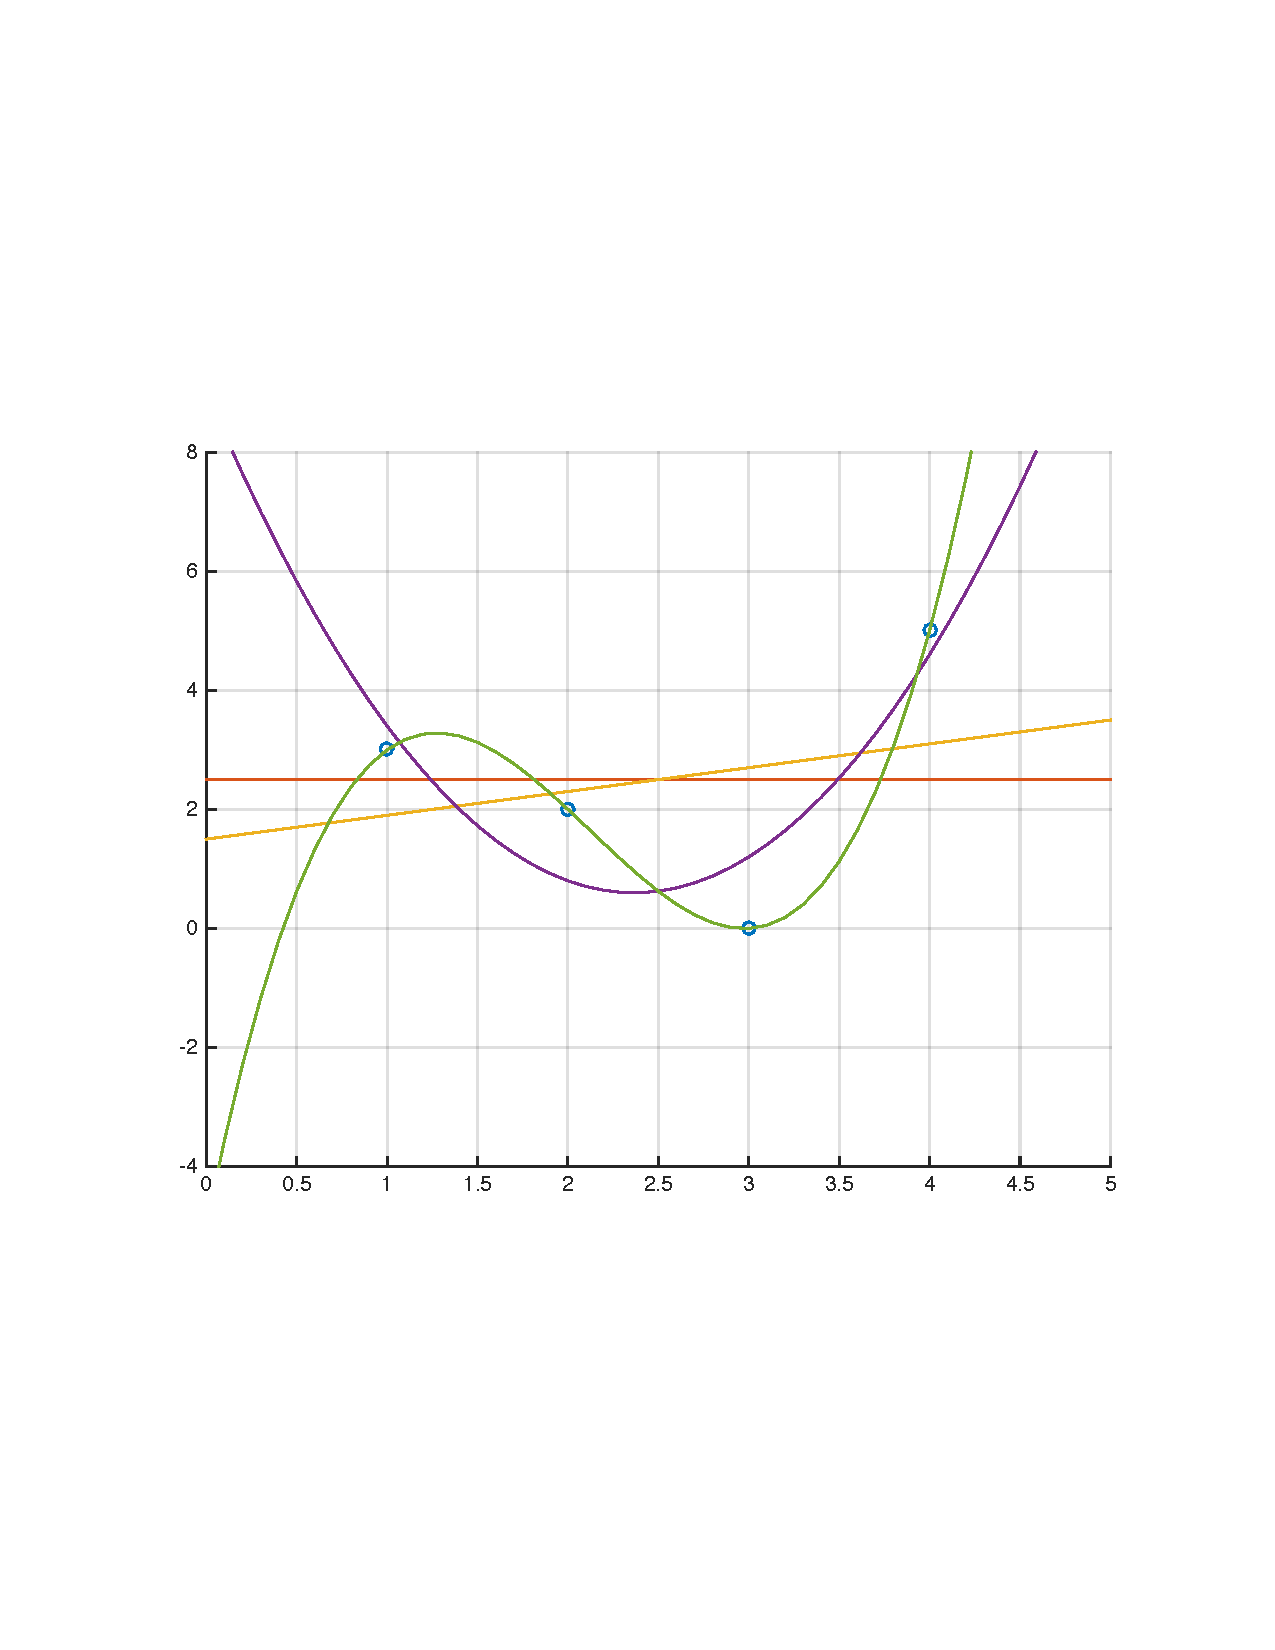
\includegraphics[width=\linewidth]{1a}
        \end{center}
        
    \item[b)] Looking at our calculated fits we get
        \begin{lstlisting}
>> fit1, fit2, fit3, fit4
fit1 =
    2.5000
fit2 =
    1.5000
    0.4000
fit3 =
    9.0000
   -7.1000
    1.5000
fit4 =
   -5.0000
   15.1667
   -8.5000
    1.3333
        \end{lstlisting}
        That is,\\
        for $k=1$ the fit is $2.5$,\\
        for $k=2$ the fit is $0.4 + 1.5x$,\\
        for $k=3$ the fit is $9 + -7.1x + 1.5x^2$,\\
        and for $k=4$ the fit is $-5 + 15.17x - 8.5x^2 + 1.33x^3$
        
    \item[c)] We can find the MSE of each of the fits by defining an MSE function and passing the fits. So we do:
        \begin{lstlisting}
mymse = @(X, w, y) (X*w - y).' * (X*w - y) / size(X, 1);
mse1 = mymse(applybasis(X, polybasis(1)), fit1, y)
mse2 = mymse(applybasis(X, polybasis(2)), fit2, y)
mse3 = mymse(applybasis(X, polybasis(3)), fit3, y)
mse4 = mymse(applybasis(X, polybasis(4)), fit4, y)
        \end{lstlisting}
        Which produces:
        \begin{lstlisting}
mse1 =
    3.2500
mse2 =
    3.0500
mse3 =
    0.8000
mse4 =
   5.1473e-29
        \end{lstlisting}       
        
\end{itemize}

\section{Overfitting}
\begin{itemize}
    \item[a)]
        We can write the function simply as (the anonymous function):
        \begin{lstlisting}
% normaldist enables us to sample from any normal distribution
normaldist = @(mean, stddeviation) randn(1)*stddeviation + mean;
        \end{lstlisting}
        
    \item[b)]
        \begin{itemize}
            \item[i)]
                We define $g_\sigma$ and $g_0.07$ and generate the data. 
                \begin{lstlisting}
% The underlying function is sin^2(2*pi*x)
func = @(x) (sin(2*pi*x))^2;

% g lets us add 0-mean normal noise to the function
g = @(x, sigma) func(x) + normaldist(0, sigma);

% g07 adds normal noise with standard deviation 0.07
g07 = @(x) g(x, 0.07);

% Random samples are generated
SX = rand([30 1]);
SY = arrayfun(g07, SX);

%i) plot the underlying function and the random noisy samples
figure
hold on
axis([0 1 -0.5 1.5])

domain = [0:0.01:1];
range = arrayfun(func, domain);
plot(domain, range, '--r');
scatter(SX, SY);
legend('Underlying function', 'Noisy Samples');
                \end{lstlisting}
                Which produces the plot
                \begin{center}
                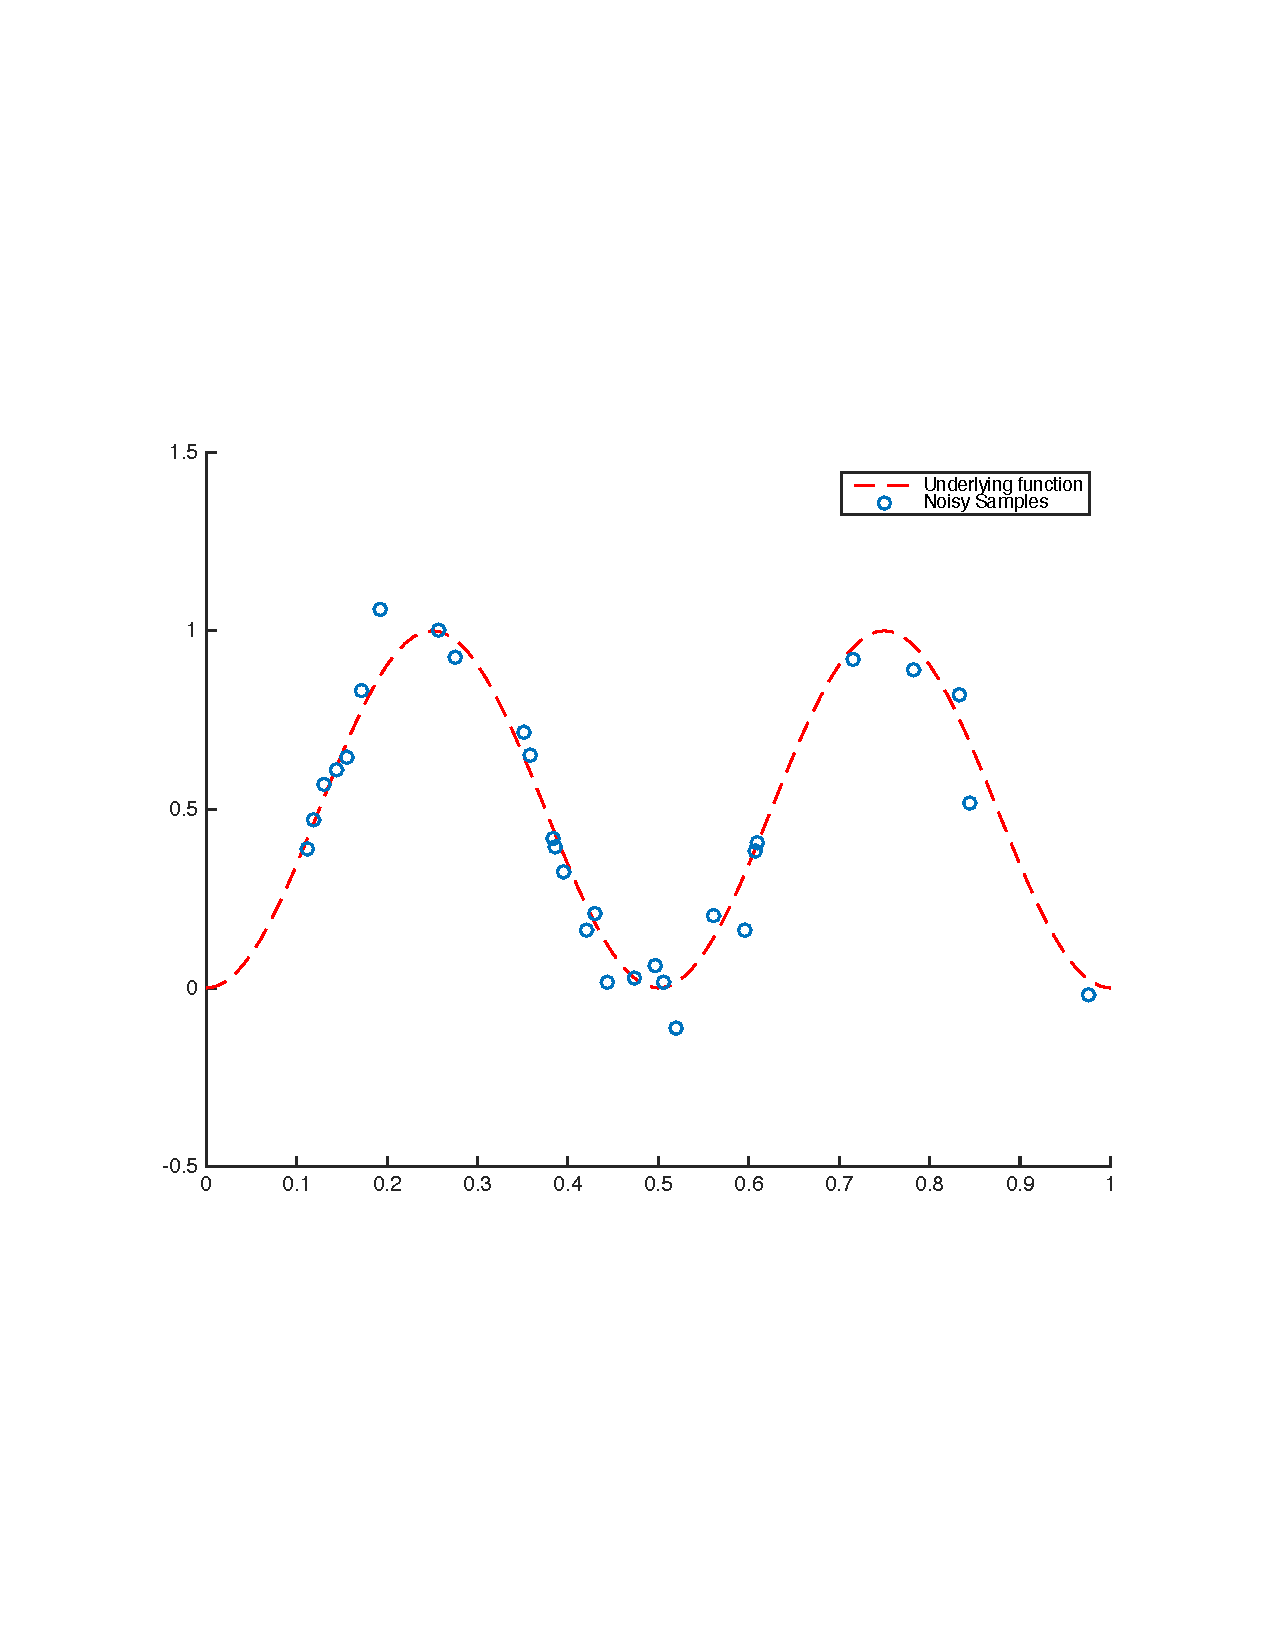
\includegraphics[width=\linewidth]{2ai}
                \end{center}
            
            \item[ii)] We fit the polynomial bases as before.
                \begin{lstlisting}
fit2 = applybasis(SX, polybasis(2))\SY;
fit5 = applybasis(SX, polybasis(5))\SY;
fit10 = applybasis(SX, polybasis(10))\SY;
fit14 = applybasis(SX, polybasis(14))\SY;
fit18 = applybasis(SX, polybasis(18))\SY;

plot(domain, applyfit(domain, polybasis(2), fit2));
plot(domain, applyfit(domain, polybasis(5), fit5));
plot(domain, applyfit(domain, polybasis(10), fit10));
plot(domain, applyfit(domain, polybasis(14), fit14));
plot(domain, applyfit(domain, polybasis(18), fit18));
legend('Underlying function', 'Noisy Samples', 'Degree 2 polynomial', 'Degree 5 polynomial', 'Degree 10 polynomial', 'Degree 14 polynomial', 'Degree 18 polynomial');
hold off
                \end{lstlisting}
                Which produces the plot
                \begin{center}
                    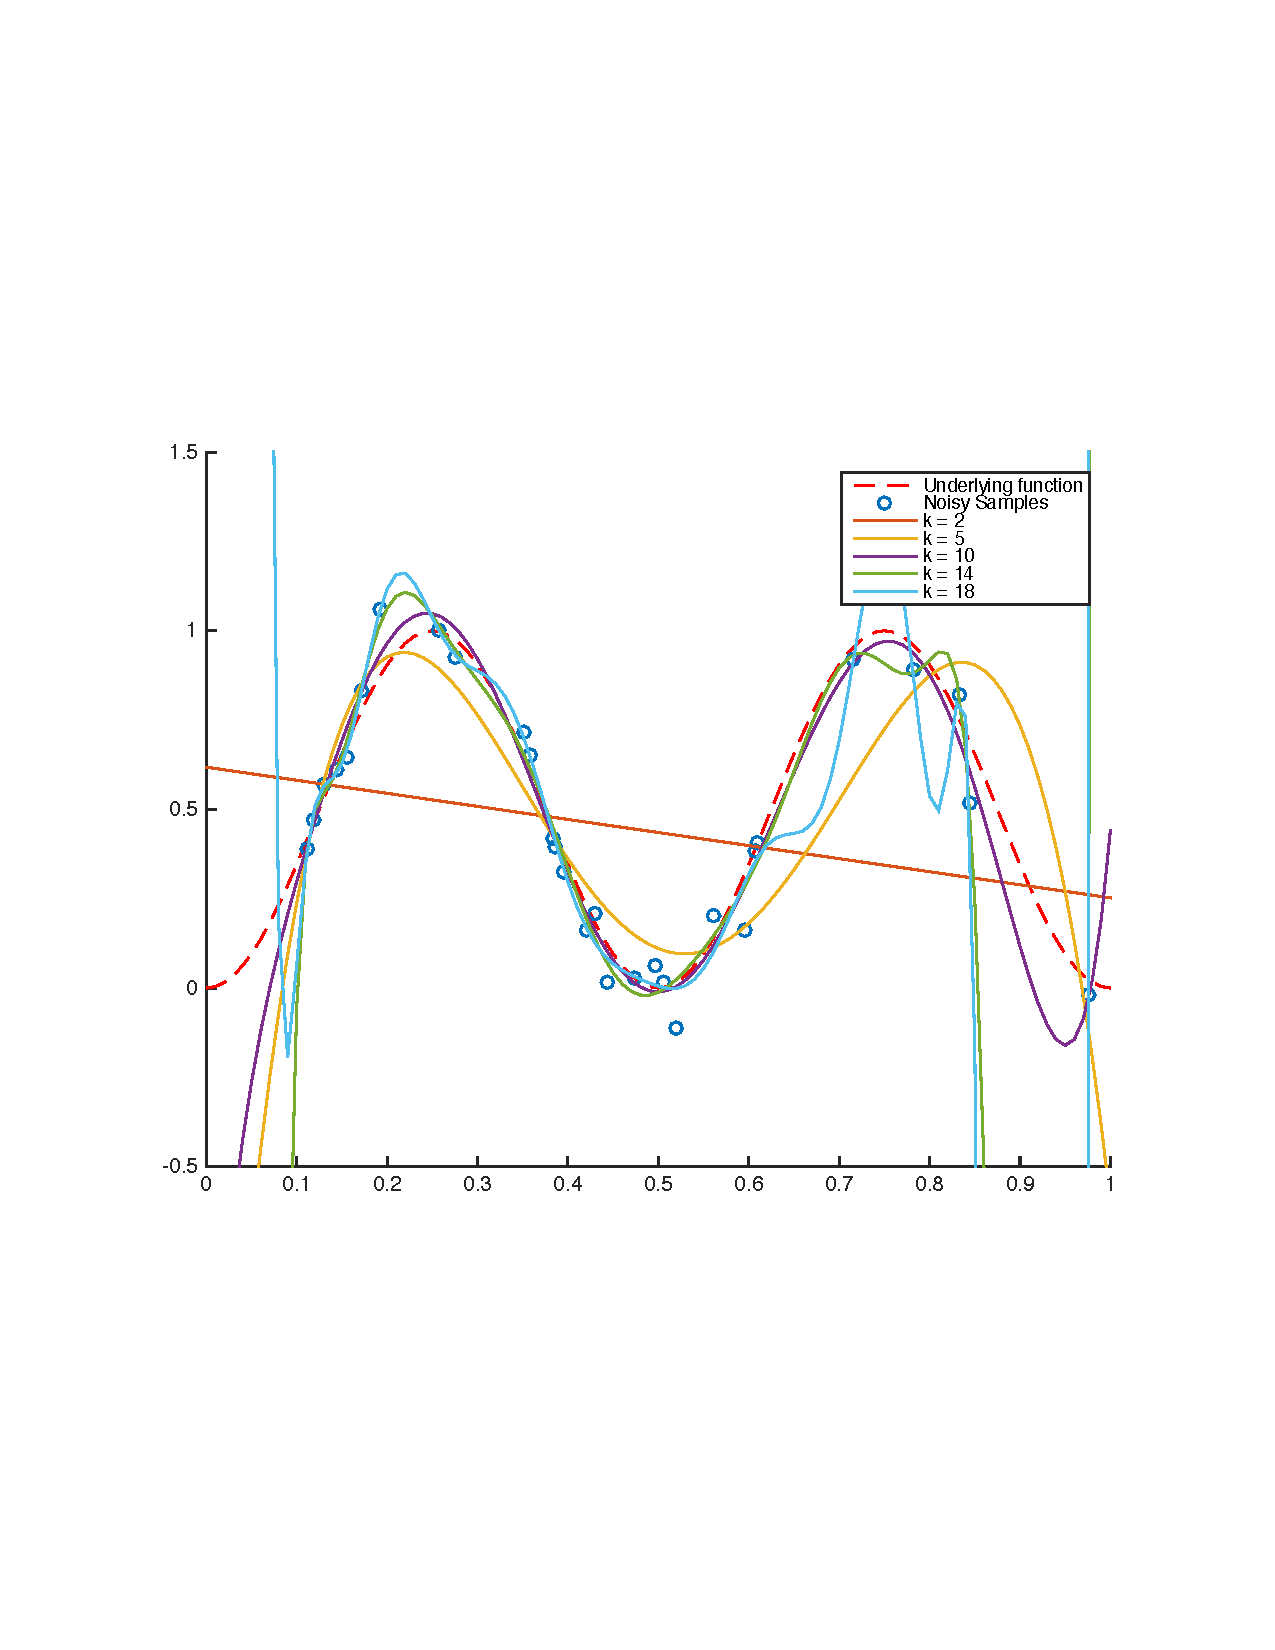
\includegraphics[width=\linewidth]{2aii}
                \end{center}



        \end{itemize}
    
    \item[c)]
        We fit for all $k=1, ..., 18$ while measuring the error for each fit. The log of the errors are plotted. In matlab:
        \begin{lstlisting}
ks = [];
errors = [];
for i = 1:18
    ks = [ks i];
    featurespacedX = applybasis(SX, polybasis(i));
    fit = featurespacedX\SY;
	errors = [errors mymse(featurespacedX, fit, SY)];
end

figure 
hold on
plot(ks, log(errors));
        \end{lstlisting}
        
        Which produces the plot
        \begin{center}
            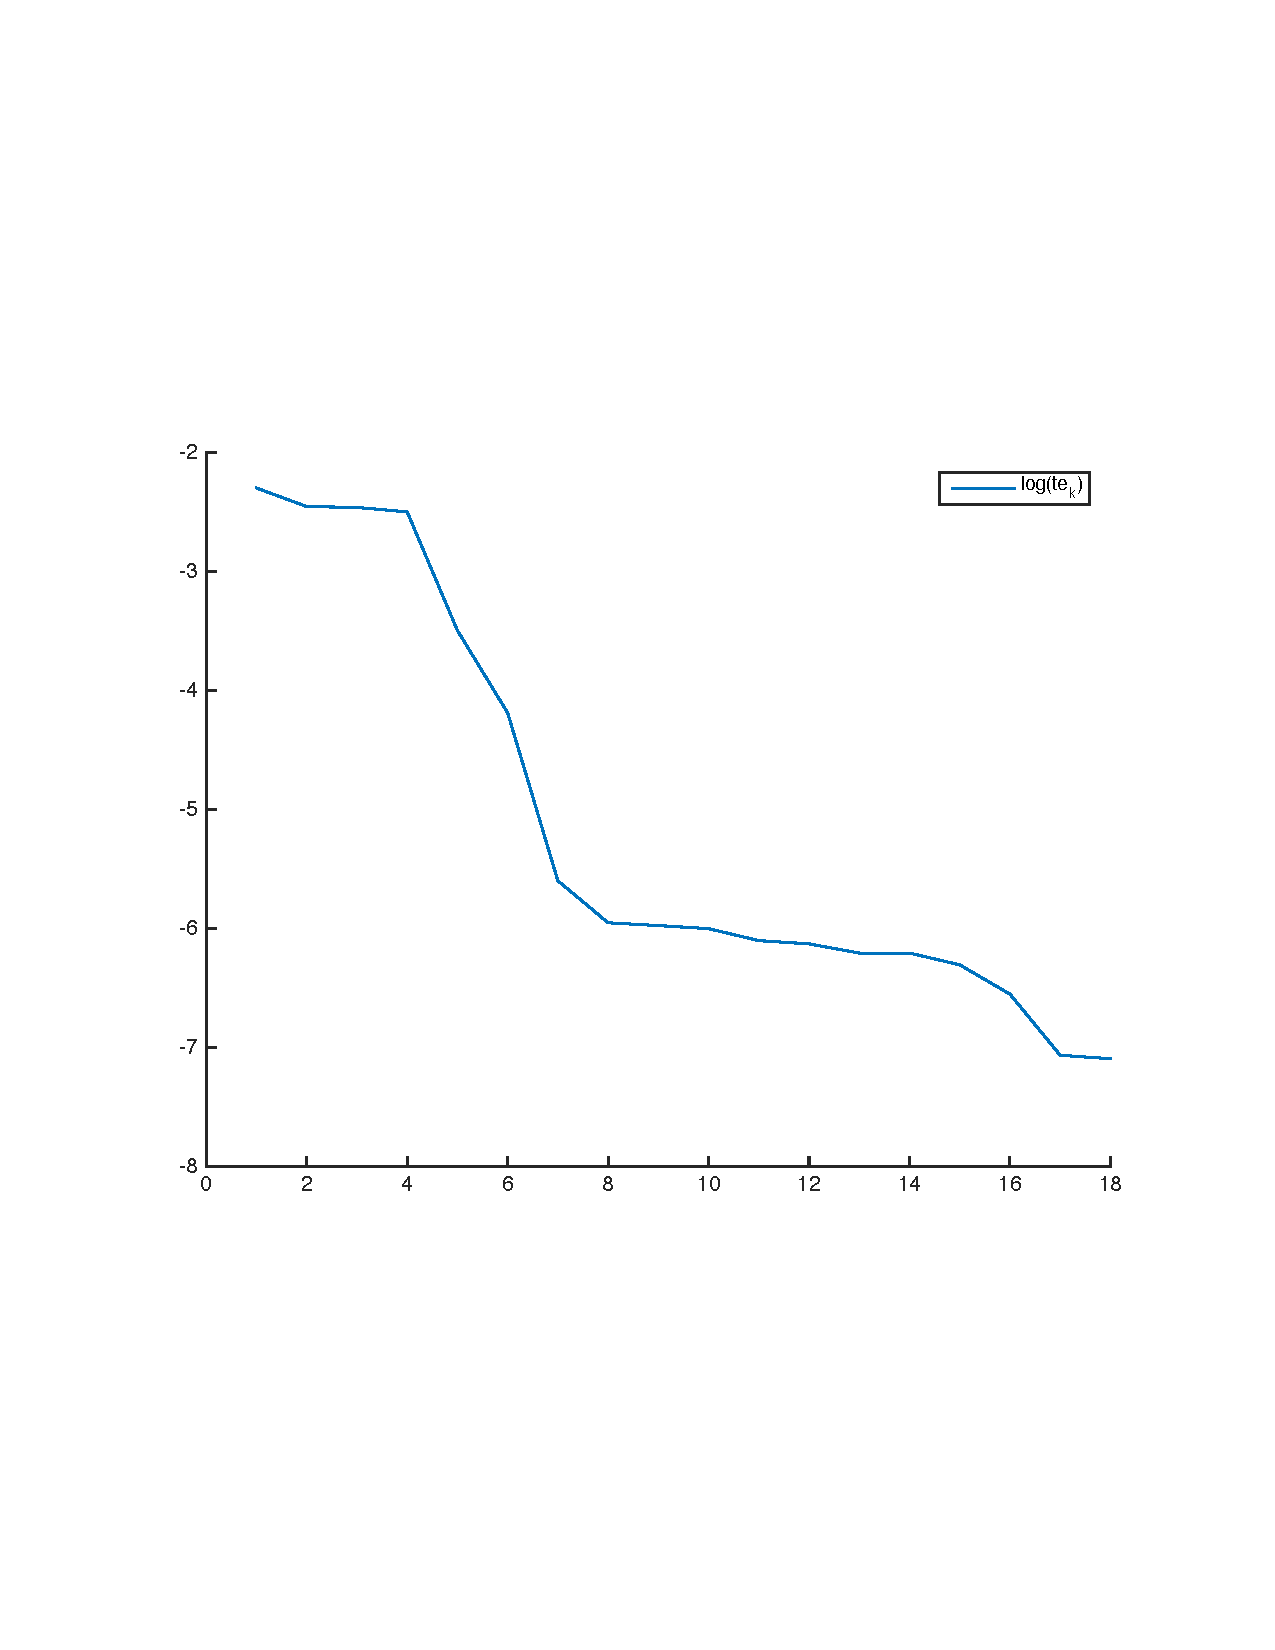
\includegraphics[width=\linewidth]{2c}
        \end{center}
    
    \item[d)] We generate 1000 test set points in the same way we generated the training set. Then we then define $tse_k$ and plot the log of it over $k=1, ..., 18$. In matlab:
        \begin{lstlisting}
% Test set generation
TX = rand([1000 1]);
TY = arrayfun(g07, TX);

% Maps input X to k-degree polynomial basis space
mappolyspace = @(X, k) applybasis(X, polybasis(k));

% Fits a k-degree polynomial to X, Y
fitpoly = @(X, Y, k) mappolyspace(X, k)\Y;

% Fits a k-degree polynomial to training set and gives test set error.
tsek = @(trainX, trainY, testX, testY, k) ...
            mymse(mappolyspace(testX, k), fitpoly(trainX, trainY, k), testY);

ks = [1:18];
errors = arrayfun(@(k) tsek(SX, SY, TX, TY, k), ks);

plot(ks, log(errors));
legend('log(te_k)', 'log(tse_k)');
hold off
        \end{lstlisting}
        
        This gives us the plot
        \begin{center}
            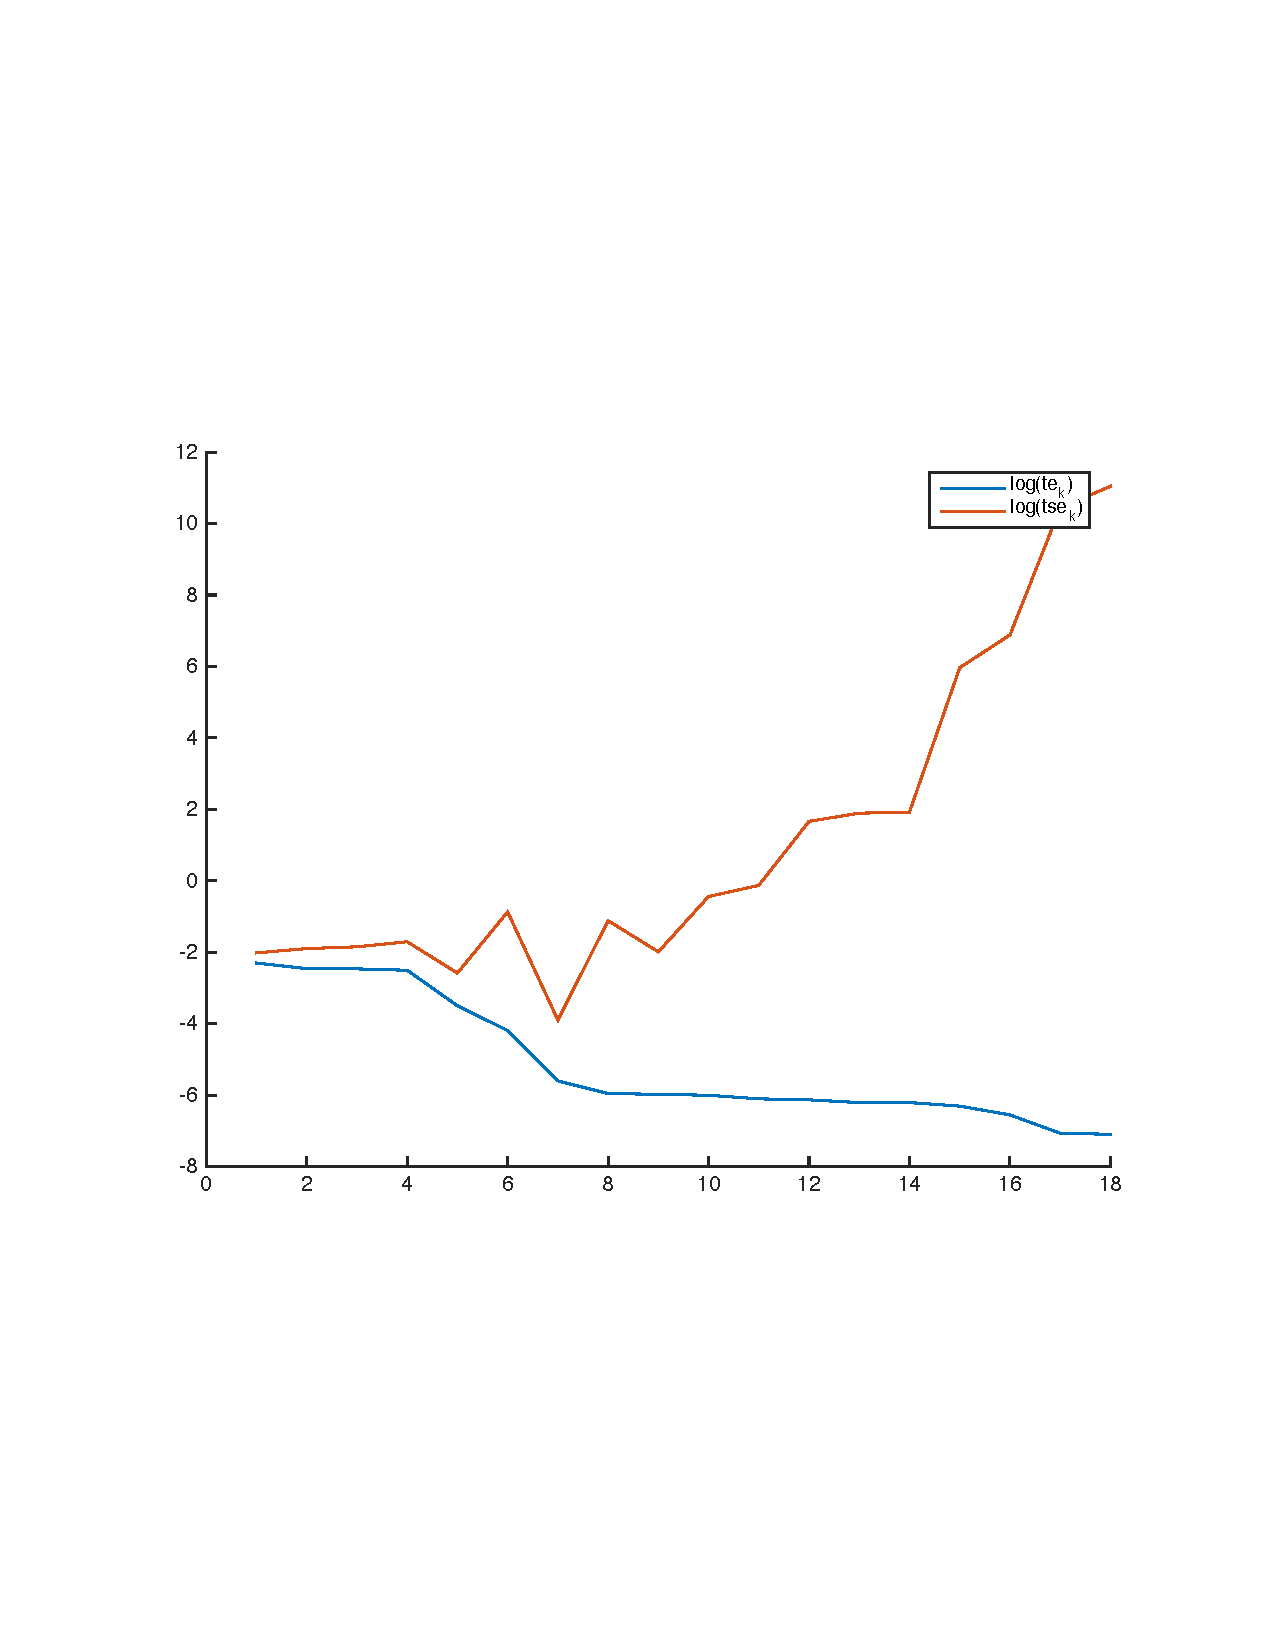
\includegraphics[width=\linewidth]{2d}
        \end{center}
    
    
    \item[e)] We generate a training set and a test set, fit the polynomials to the training set, and record the error on both the training set and the test set. We do this 100 times and plot the average errors.
        
        \begin{lstlisting}
iterations = 100;
totaltrainerrors = 0;
totaltesterrors = 0;
ks = [1:18];

for i = 1:iterations
    SX = rand([30 1]);
    SY = arrayfun(g07, SX);
    TX = rand([1000 1]);
    TY = arrayfun(g07, TX);
    
    trainerrors = arrayfun(@(k) tsek(SX, SY, SX, SY, k), ks);
    testerrors = arrayfun(@(k) tsek(SX, SY, TX, TY, k), ks);
    
    totaltrainerrors = totaltrainerrors + trainerrors;
    totaltesterrors = totaltesterrors + testerrors;
end

avgtrainerror = totaltrainerrors/iterations;
avgtesterror = totaltesterrors/iterations;

figure
hold on
plot(ks, log(avgtrainerror));
plot(ks, log(avgtesterror));
legend('Avg. training error', 'Avg. test error');
hold off
        \end{lstlisting}

        This produces the plot
        \begin{center}
        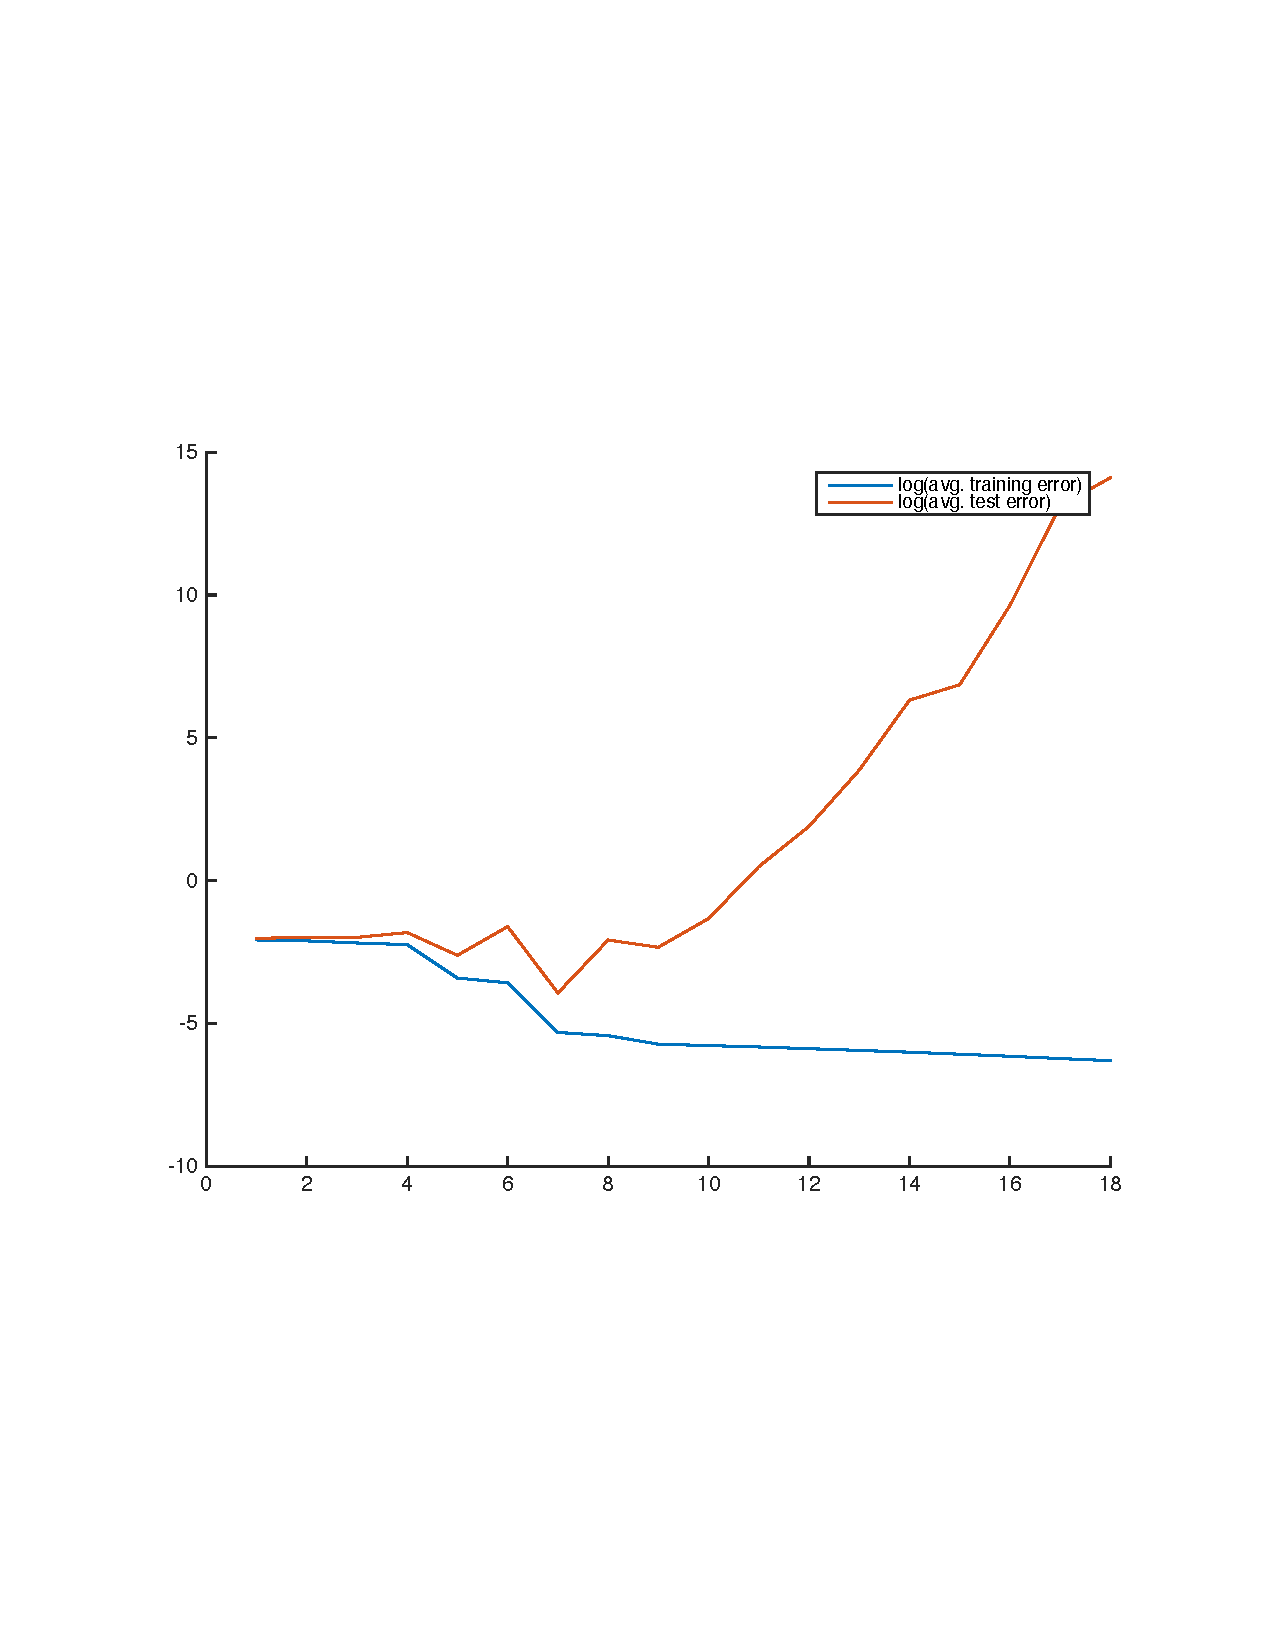
\includegraphics[width=\linewidth]{2e}
        \end{center}

\end{itemize}
\section{Repeat 2 (c-e) with sine basis}
    The basis is $\sin( 1 \pi x), \sin( 2 \pi x), \sin(3 \pi x), . . . , \sin(k \pi x)$.

\begin{itemize}
    \item[c \& d)] To repeat the experiment with this different basis we simply define the new basis (see appendix \ref{appendix:sinbasis}), and redefine $tse_k$ with this new type of basis. A new test and training set is generated and we fit the $k=1, ..., 18$ functions to the training set. The error on the training and test sets over $k=1, ..., 18$ is plotted. In matlab:
    \begin{lstlisting}
%c & d)
% Maps input X to the {sin(1*pi*x), ..., sin(k*pi*x)} basis space
mapsinspace = @(X, k) applybasis(X, sinbasis(k));

% Fits a the the data in the sinus space
fitsin = @(X, Y, k) mapsinspace(X, k)\Y;

% Fits the training set in the sin space and gives test set error.
tsek = @(trainX, trainY, testX, testY, k) ...
            mymse(mapsinspace(testX, k), fitsin(trainX, trainY, k), testY);

SX = rand([30 1]);
SY = arrayfun(g07, SX);
TX = rand([1000 1]);
TY = arrayfun(g07, TX);

ks = [1:18];
trainerrors = arrayfun(@(k) tsek(SX, SY, SX, SY, k), ks);
testerrors = arrayfun(@(k) tsek(SX, SY, TX, TY, k), ks)

figure
hold on
plot(ks, log(trainerrors));
plot(ks, log(testerrors));
legend('log(te_k)', 'log(tse_k)');
hold off
    \end{lstlisting}
    This produces the plot
    \begin{center}
        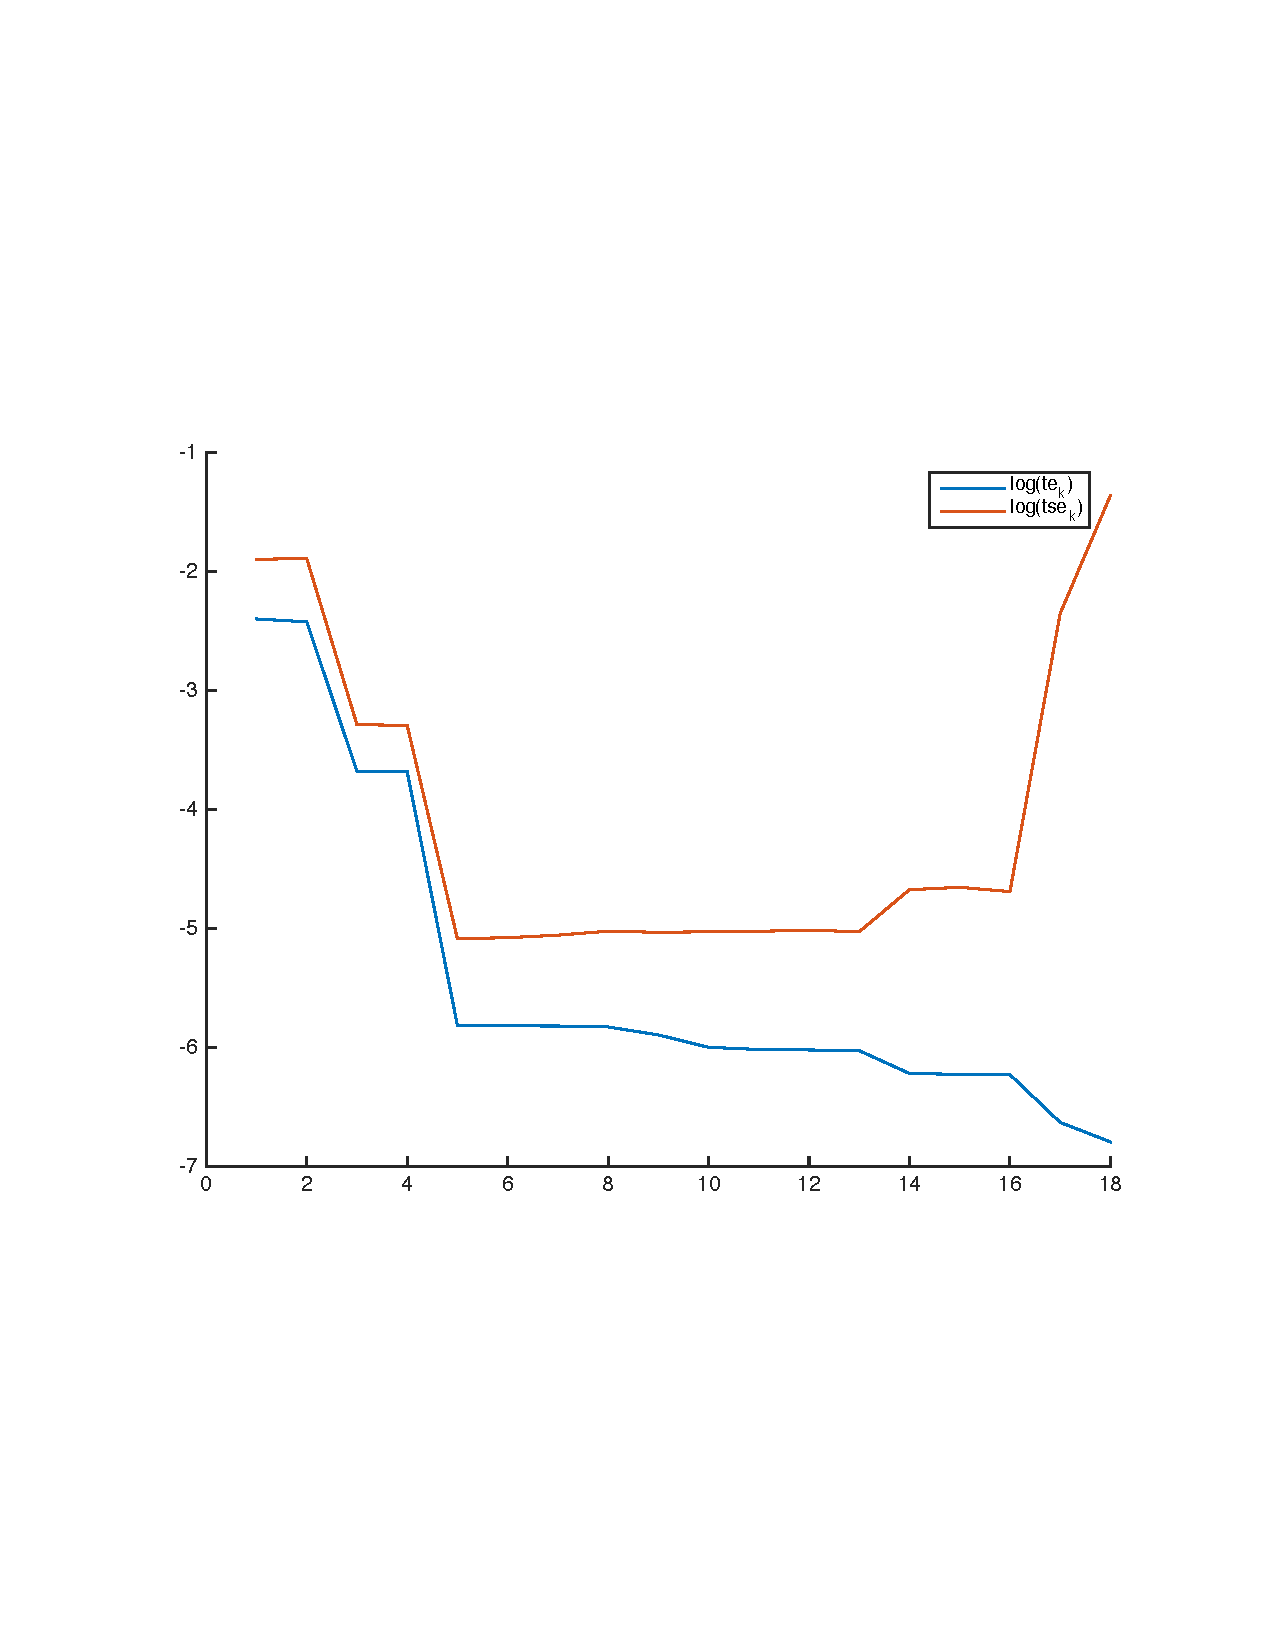
\includegraphics[width=\linewidth]{3cd}
    \end{center}
    
    \item[d)]  Again, we do this 100 times and plot the average errors on the training set and the test set. In Matlab:
        \begin{lstlisting}
iterations = 100;
totaltrainerrors = 0;
totaltesterrors = 0;
ks = [1:18];

for i = 1:iterations
    SX = rand([30 1]);
    SY = arrayfun(g07, SX);
    TX = rand([1000 1]);
    TY = arrayfun(g07, TX);
    
    trainerrors = arrayfun(@(k) tsek(SX, SY, SX, SY, k), ks);
    testerrors = arrayfun(@(k) tsek(SX, SY, TX, TY, k), ks);
    
    totaltrainerrors = totaltrainerrors + trainerrors;
    totaltesterrors = totaltesterrors + testerrors;
end

avgtrainerror = totaltrainerrors/iterations;
avgtesterror = totaltesterrors/iterations;

figure
hold on
plot(ks, log(avgtrainerror));
plot(ks, log(avgtesterror));
legend('Avg. training error', 'Avg. test error');
hold off
        \end{lstlisting}
        Which produces the plot
        \begin{center}
            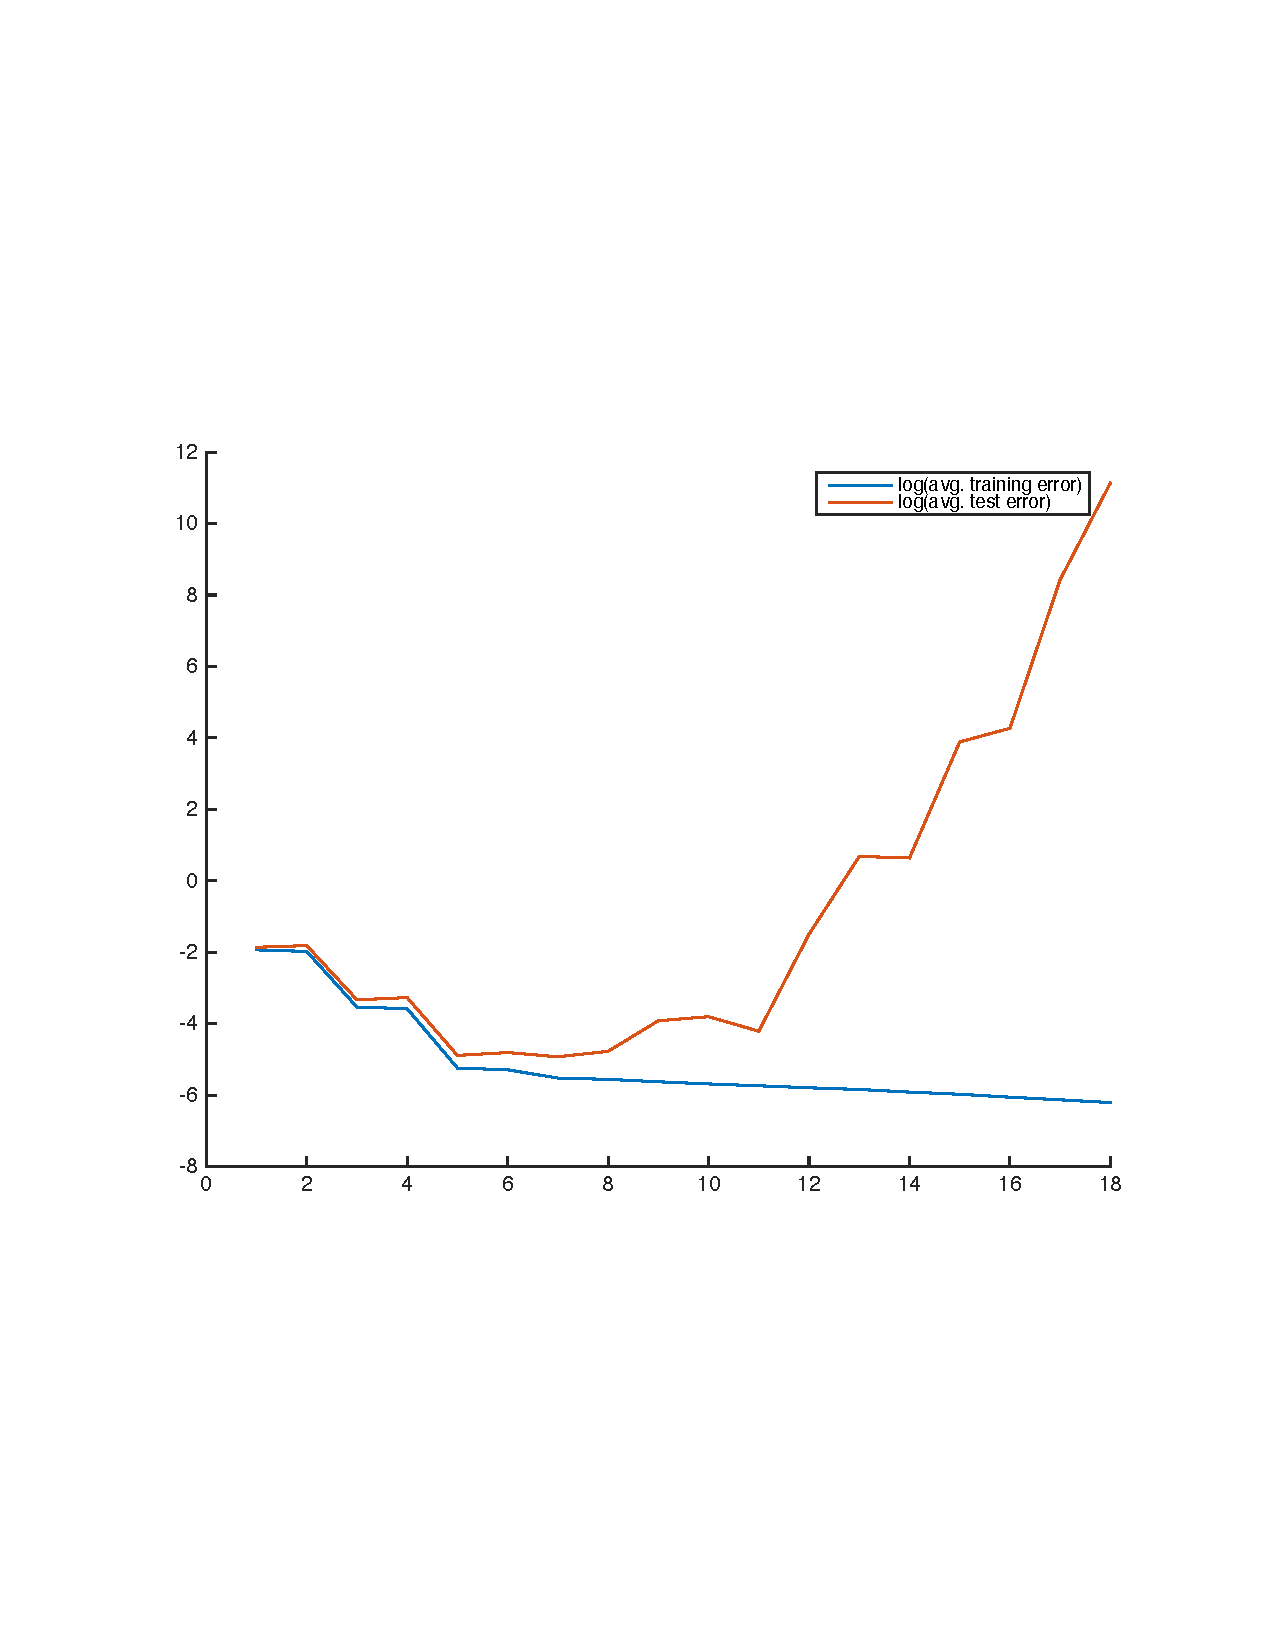
\includegraphics[width=\linewidth]{3e}
        \end{center}

\end{itemize}


\section{Appendix}
    \subsection{Implementation of applybasis}
        \begin{lstlisting}
% Applies a basis to a matrix X
function sol = applybasis(X, basis)
    % X     - (m x n) - a matrix of row input vectors
    % basis - (k x 1) - an array of functions
    % sol   - (m x k) - X with the applied basis
    
    sol = [];
    for i = 1:size(basis, 2)
        sol = [sol arrayfun(basis{i}, X)];
    end
end
        \end{lstlisting}
    
    \subsection{Implementation of applyfit}
        \begin{lstlisting}
% Applies a basis and a matching set of coefficients (the fit) to input X
% e.g. X = [1,2,3], basis = {@(x) x^2}, coefficients = [1] gives
% sol = [1, 4, 9] 
function sol = applyfit(X, basis, coefficients)
    sol = 0;
    for i = 1:size(basis, 2)
        sol = sol + coefficients(i) * basis{i}(X);
    end
end
        \end{lstlisting}
    
    \subsection{Implementation of polybasis}
        \begin{lstlisting}
% Returns a k-polynomial basis. E.g. {@(x) 1, @(x) x, @(x) x^2}
function basis = polybasis(k)
    if k <= 1
        % repmat used to enforce same dimensionality
        basis = {@(x) repmat(1, size(x,1), size(x,2))}; 
    else
        basis = [polybasis(k-1), {@(x) x.^(k-1)}];
    end
end
        \end{lstlisting}
    
    \subsection{Implementatino of sinbasis} \label{appendix:sinbasis}
        \begin{lstlisting}
% Returns the k-sine basis 
function basis = sinbasis(k)
    if k <= 1
        basis = {@(x) sin(k*pi*x)}; 
    else
        basis = [sinbasis(k-1), {@(x) sin(k*pi*x)}];
    end
end
        \end{lstlisting}


\end{document}
